\begin{tabularx}
{\textwidth}{llllll}
    % \toprule
    \textbf{Image dimensions} & \textbf{\# pos. samples} & \textbf{\# neg. samples} & \textbf{\# stages} & \textbf{Training time} \\
    % \midrule
    24x24 & 300 & 500 & 19 & \mytilda7 minutes \\
    \multicolumn{5}{c}{
        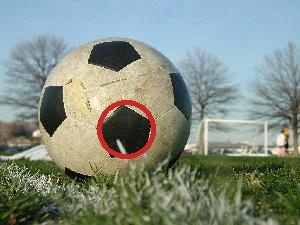
\includegraphics[width=6.0cm]{results/1/sphere_3}
        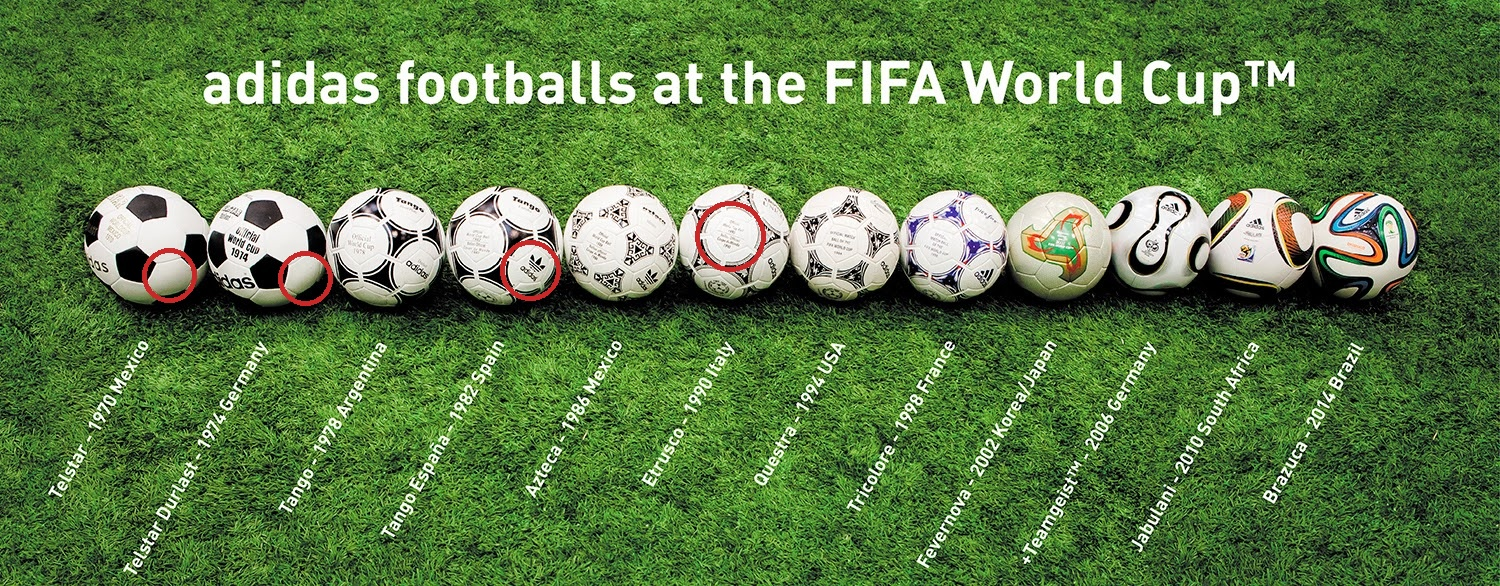
\includegraphics[width=6.0cm]{results/1/sphere_4}
        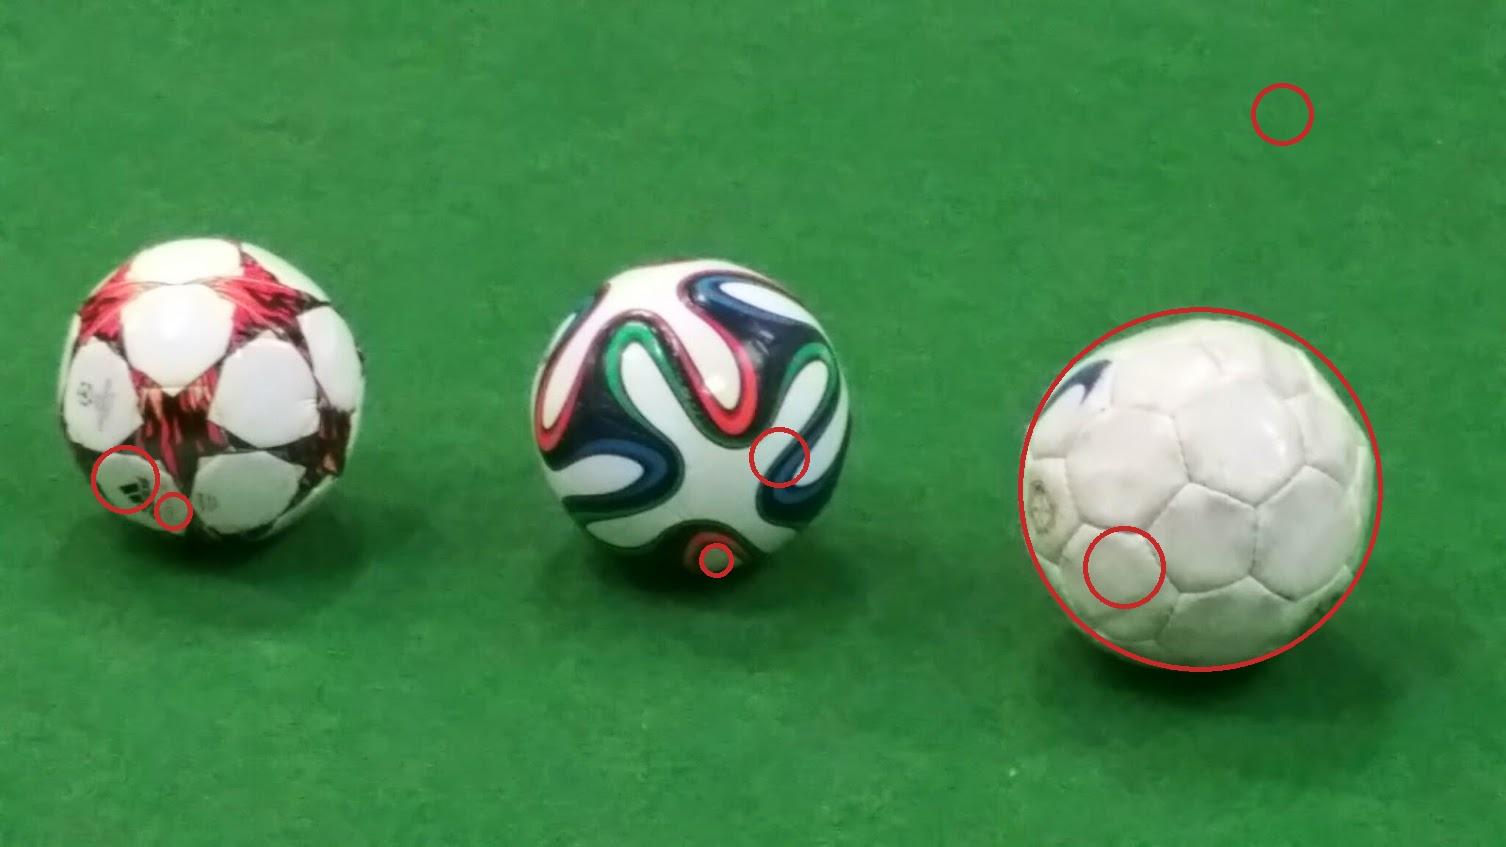
\includegraphics[width=6.0cm]{results/1/sphere_5}
    } \\
    \multicolumn{5}{c}{
        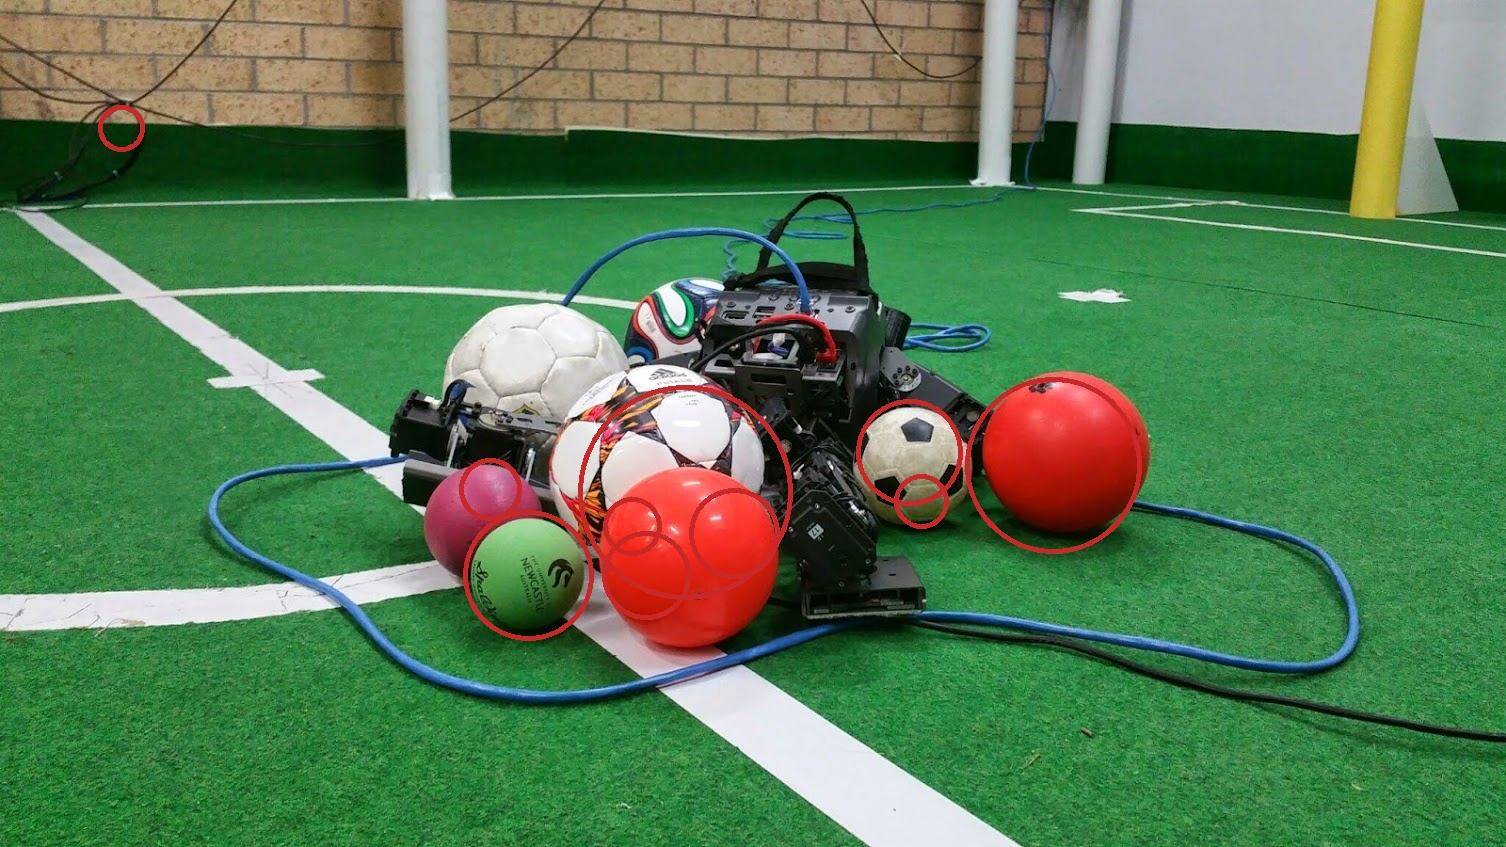
\includegraphics[width=6.0cm]{results/1/sphere_6}
        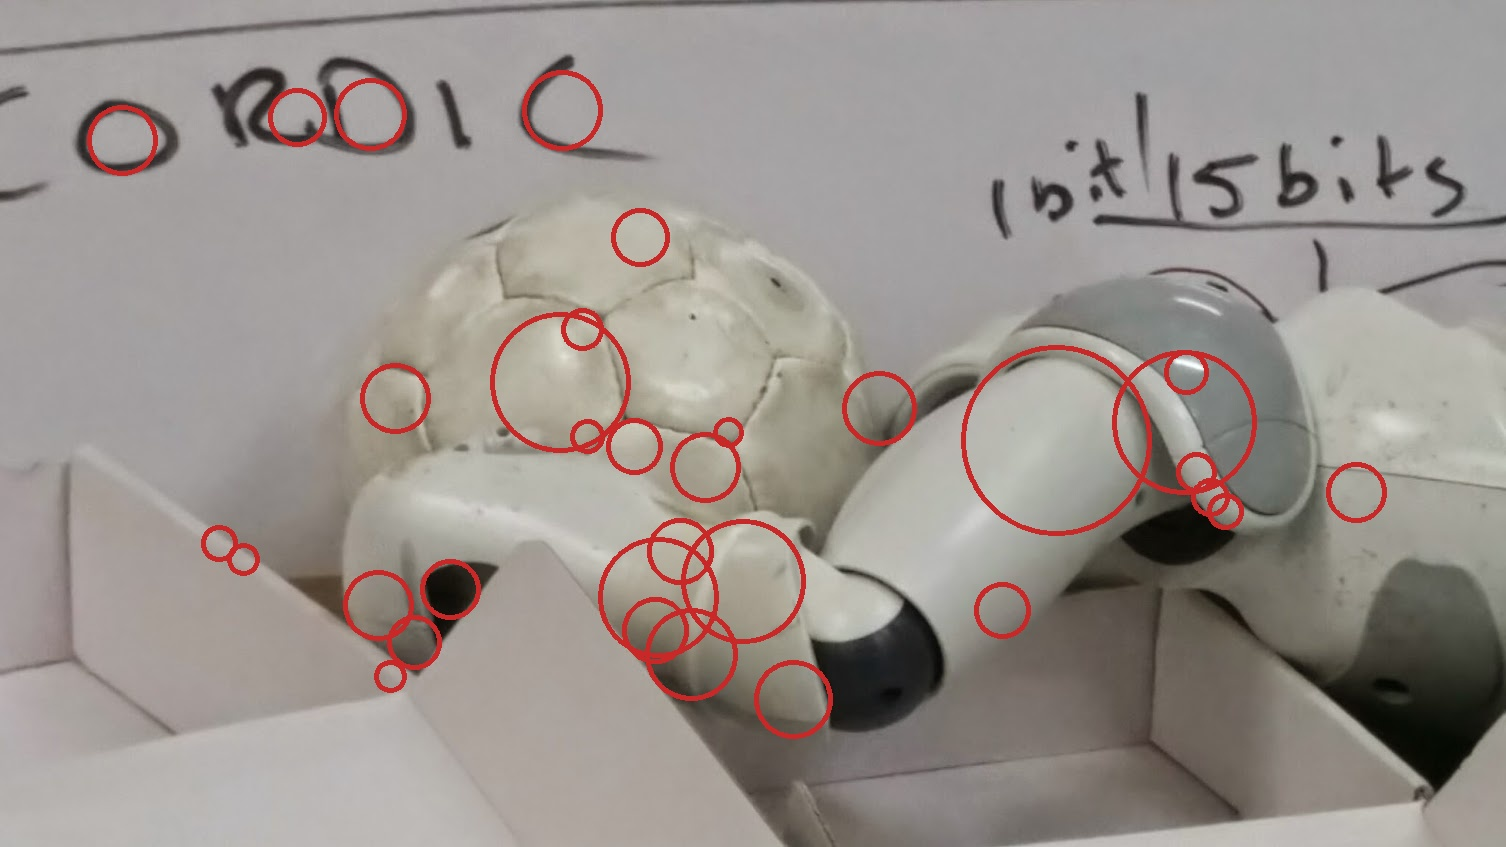
\includegraphics[width=6.0cm]{results/1/sphere_7}
        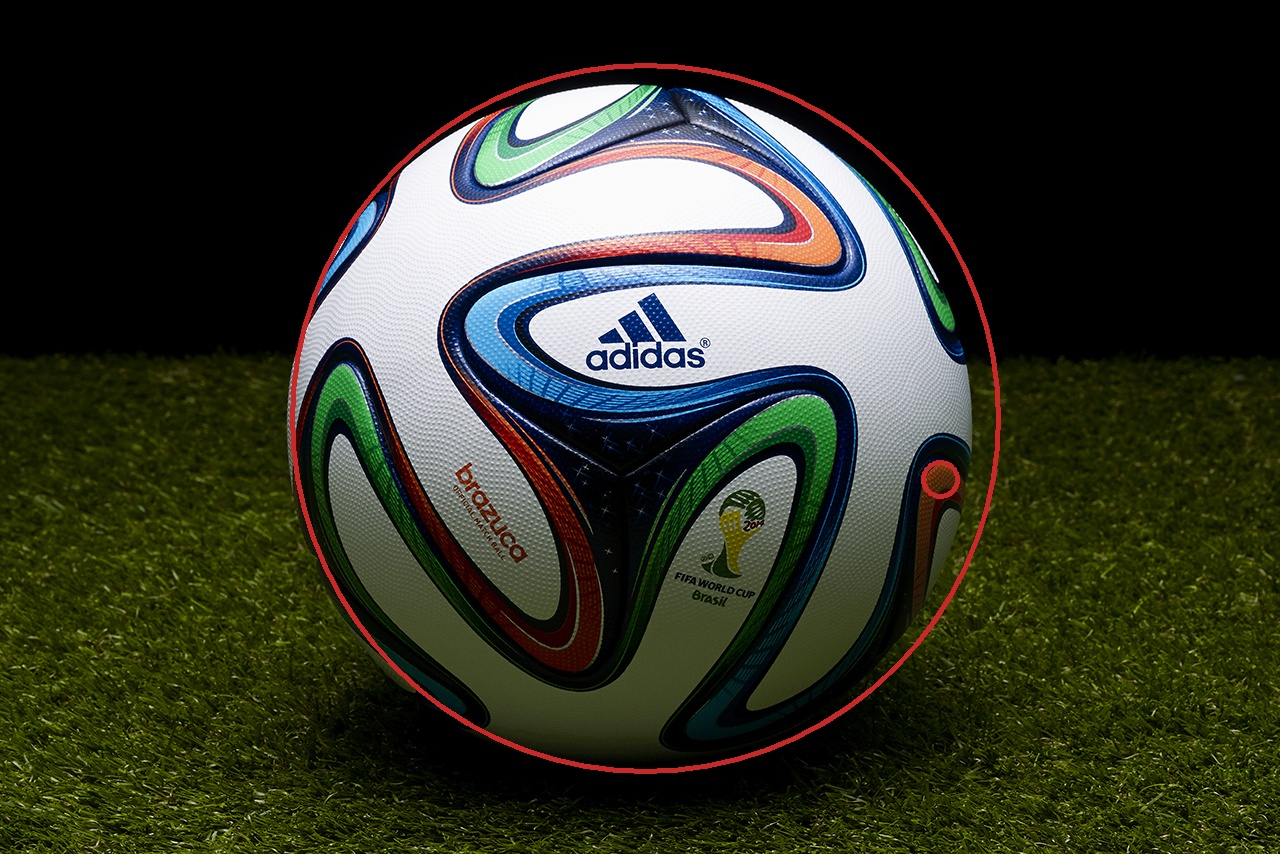
\includegraphics[width=6.0cm]{results/1/sphere_8}
    } \\
    24x24 & 500 & 1000 & 15 & \mytilda2 minutes \\
    \multicolumn{5}{c}{
        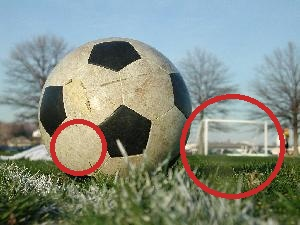
\includegraphics[width=6.0cm]{results/2/sphere_3}
        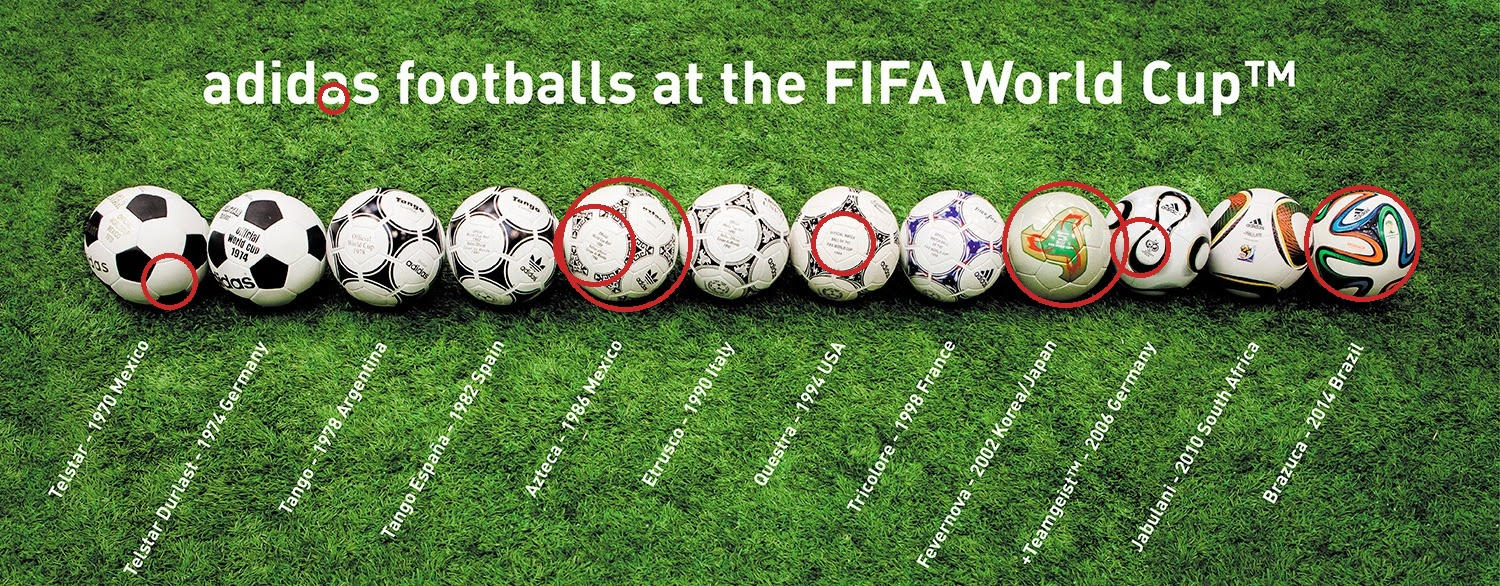
\includegraphics[width=6.0cm]{results/2/sphere_4}
        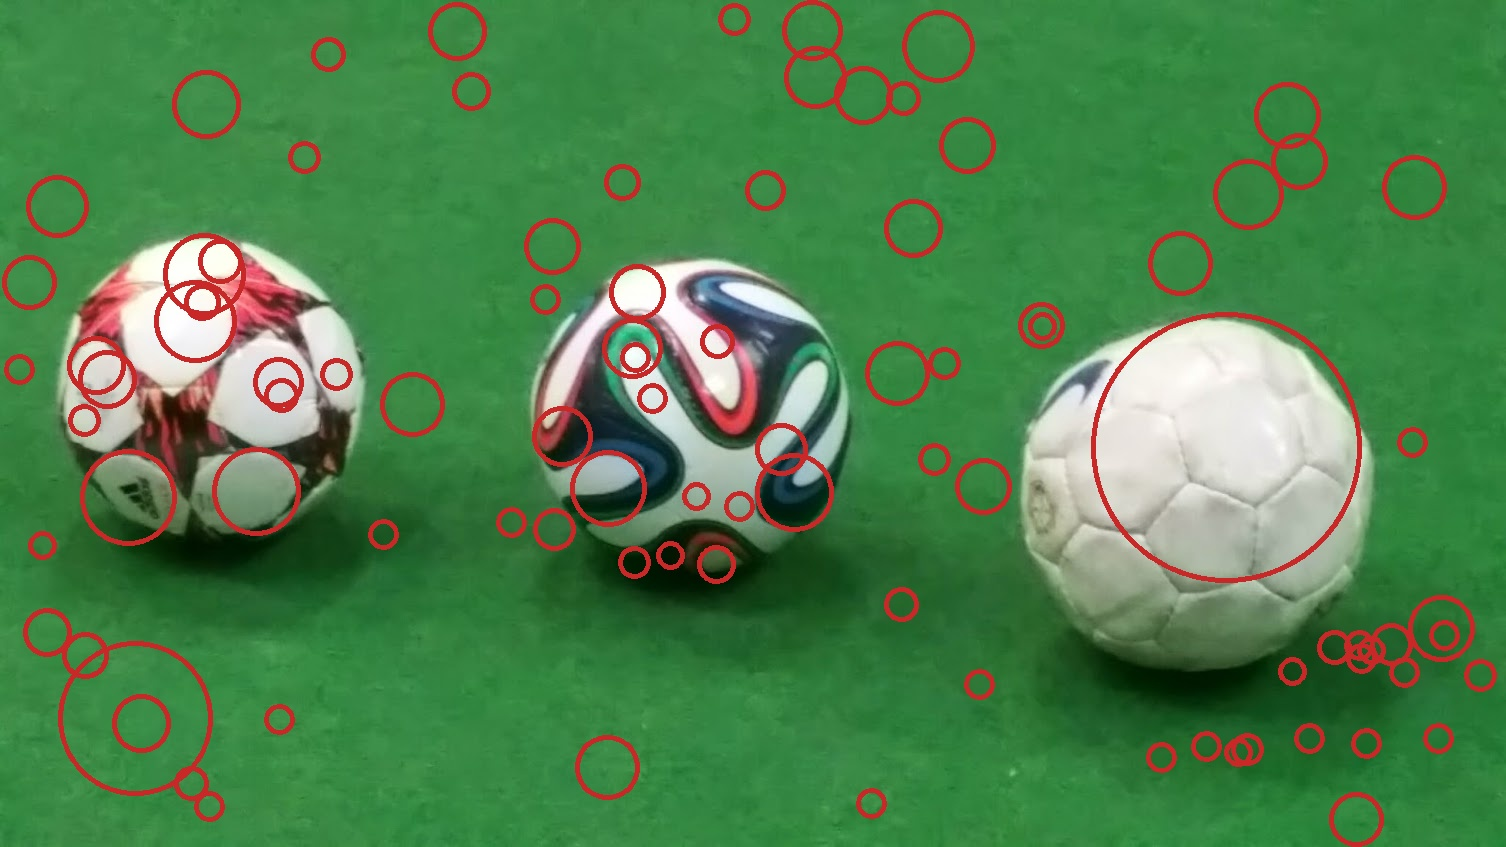
\includegraphics[width=6.0cm]{results/2/sphere_5}
    } \\
    \multicolumn{5}{c}{
        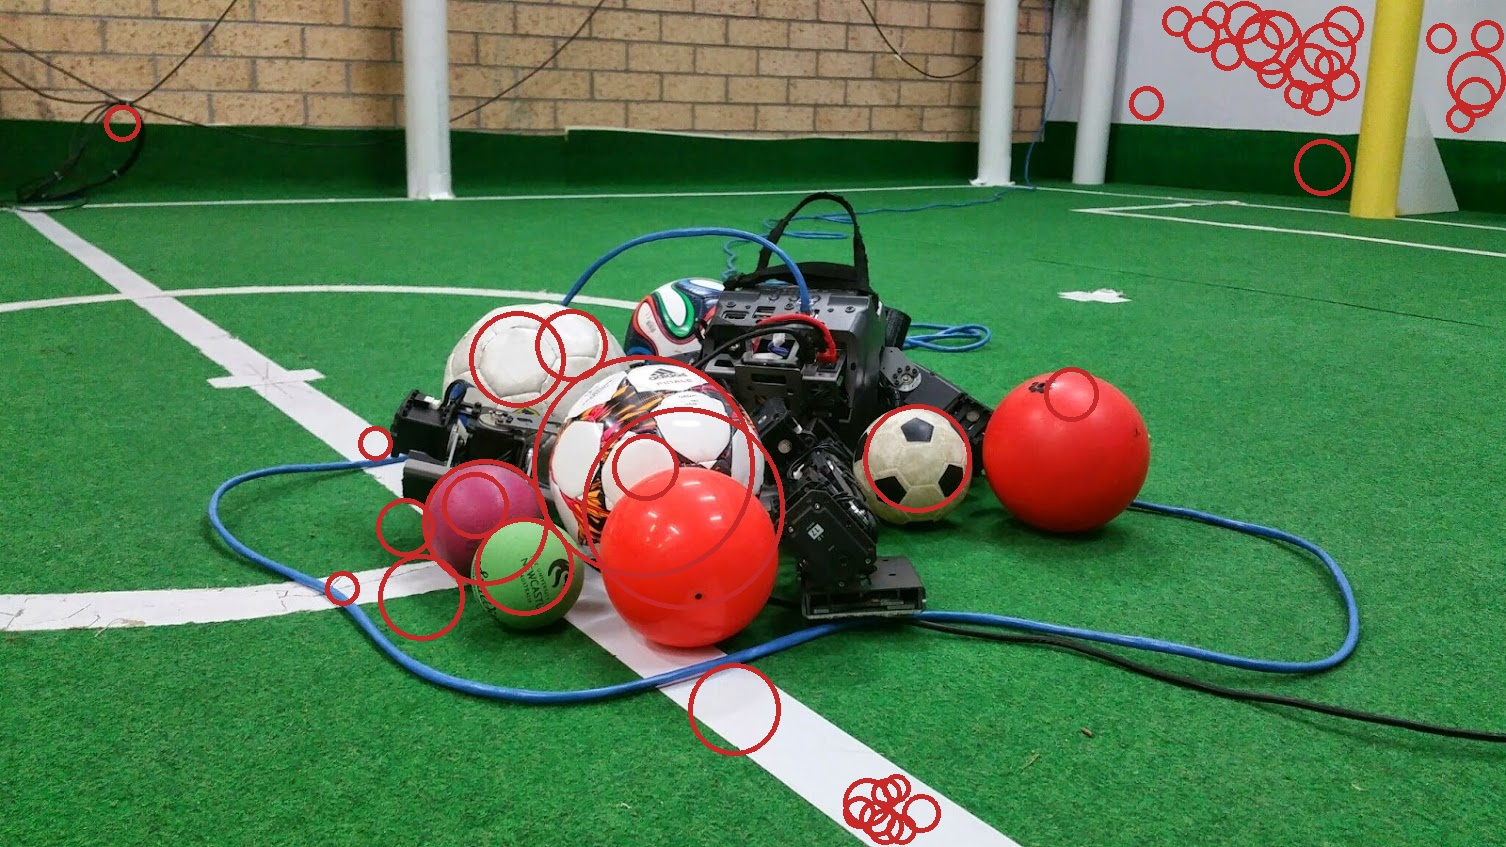
\includegraphics[width=6.0cm]{results/2/sphere_6}
        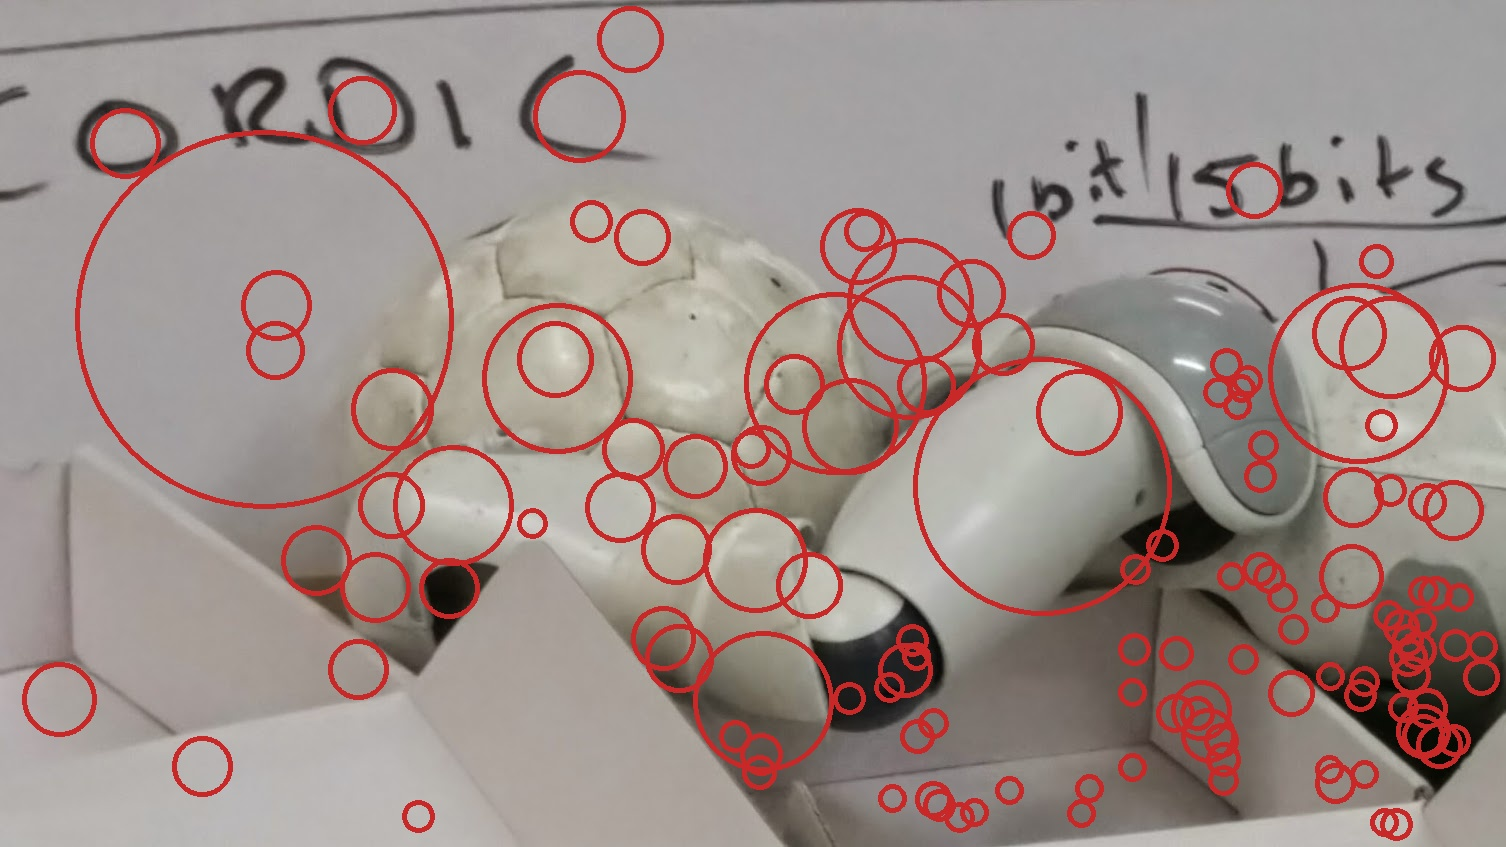
\includegraphics[width=6.0cm]{results/2/sphere_7}
        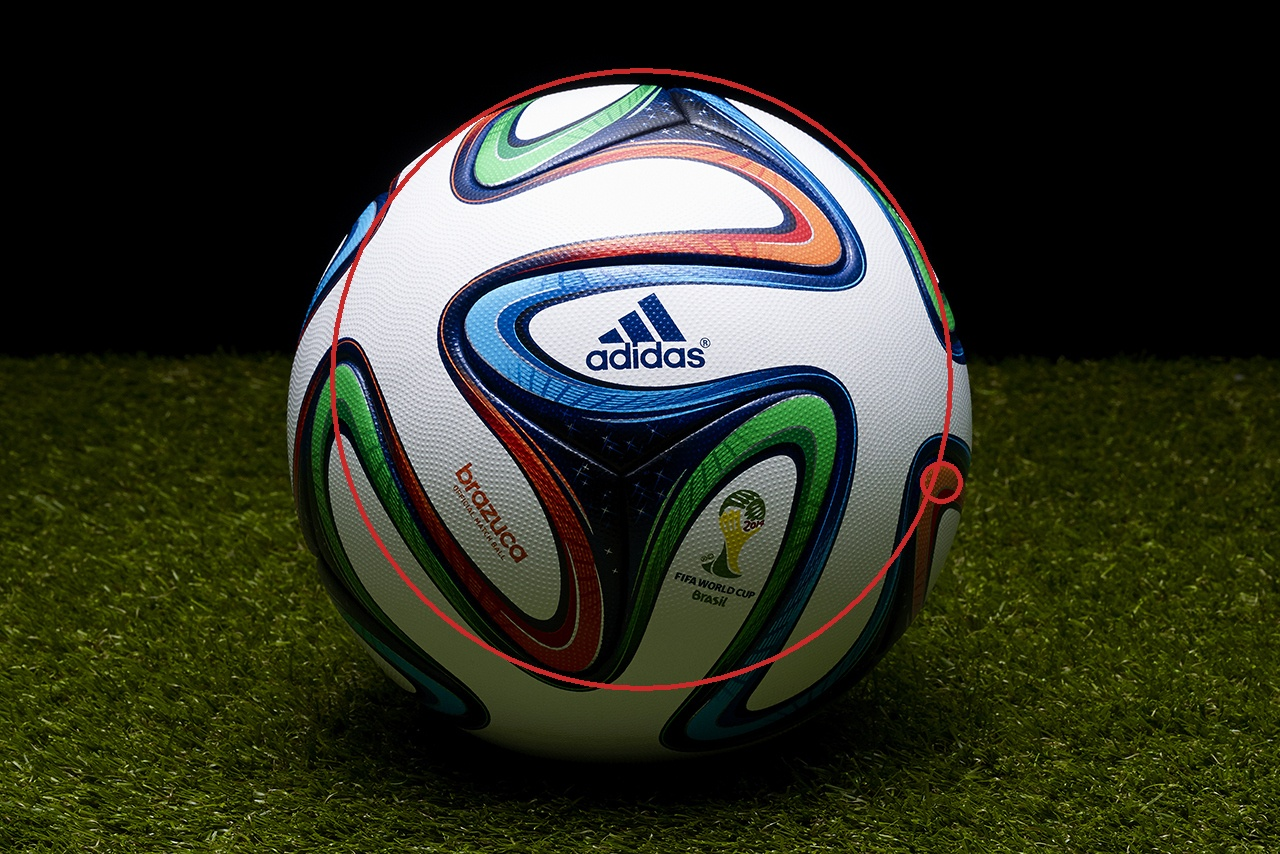
\includegraphics[width=6.0cm]{results/2/sphere_8}
    } \\
    24x24 & 600 & 1376 & 19 & \mytilda17 minutes \\
    \multicolumn{5}{c}{
        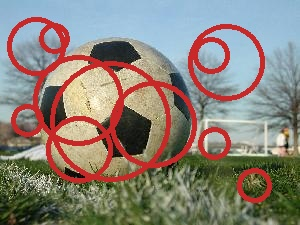
\includegraphics[width=6.0cm]{results/3/sphere_3}
        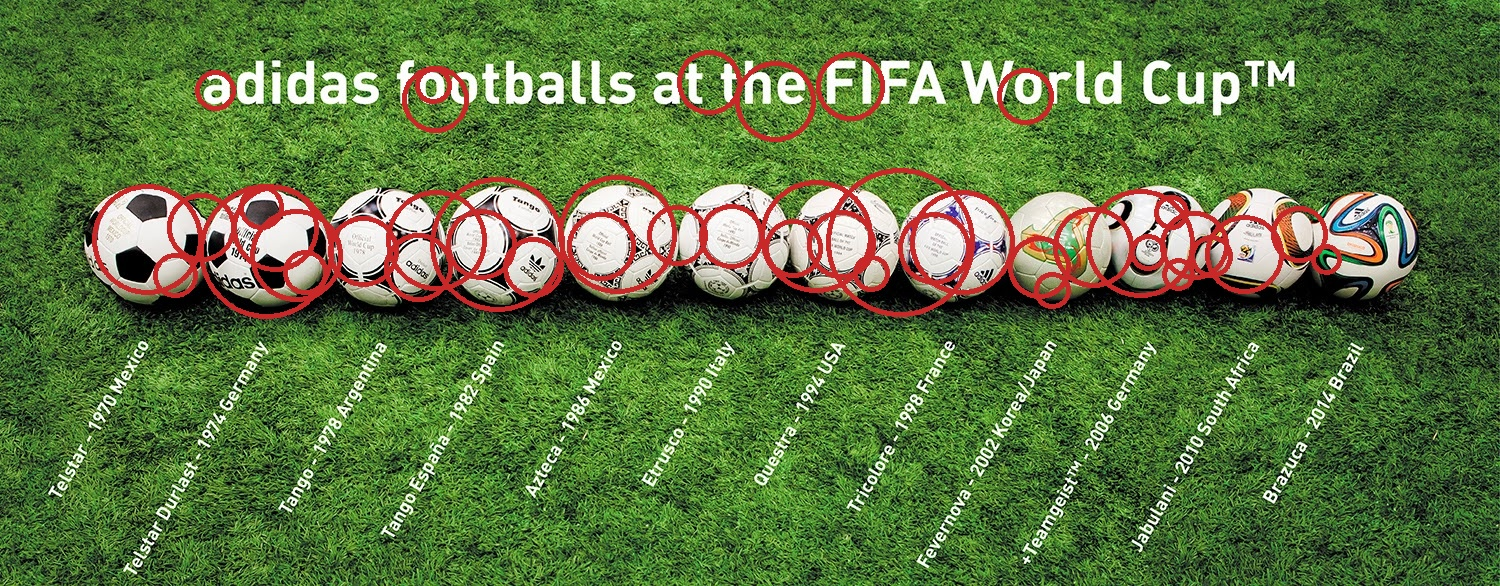
\includegraphics[width=6.0cm]{results/3/sphere_4}
        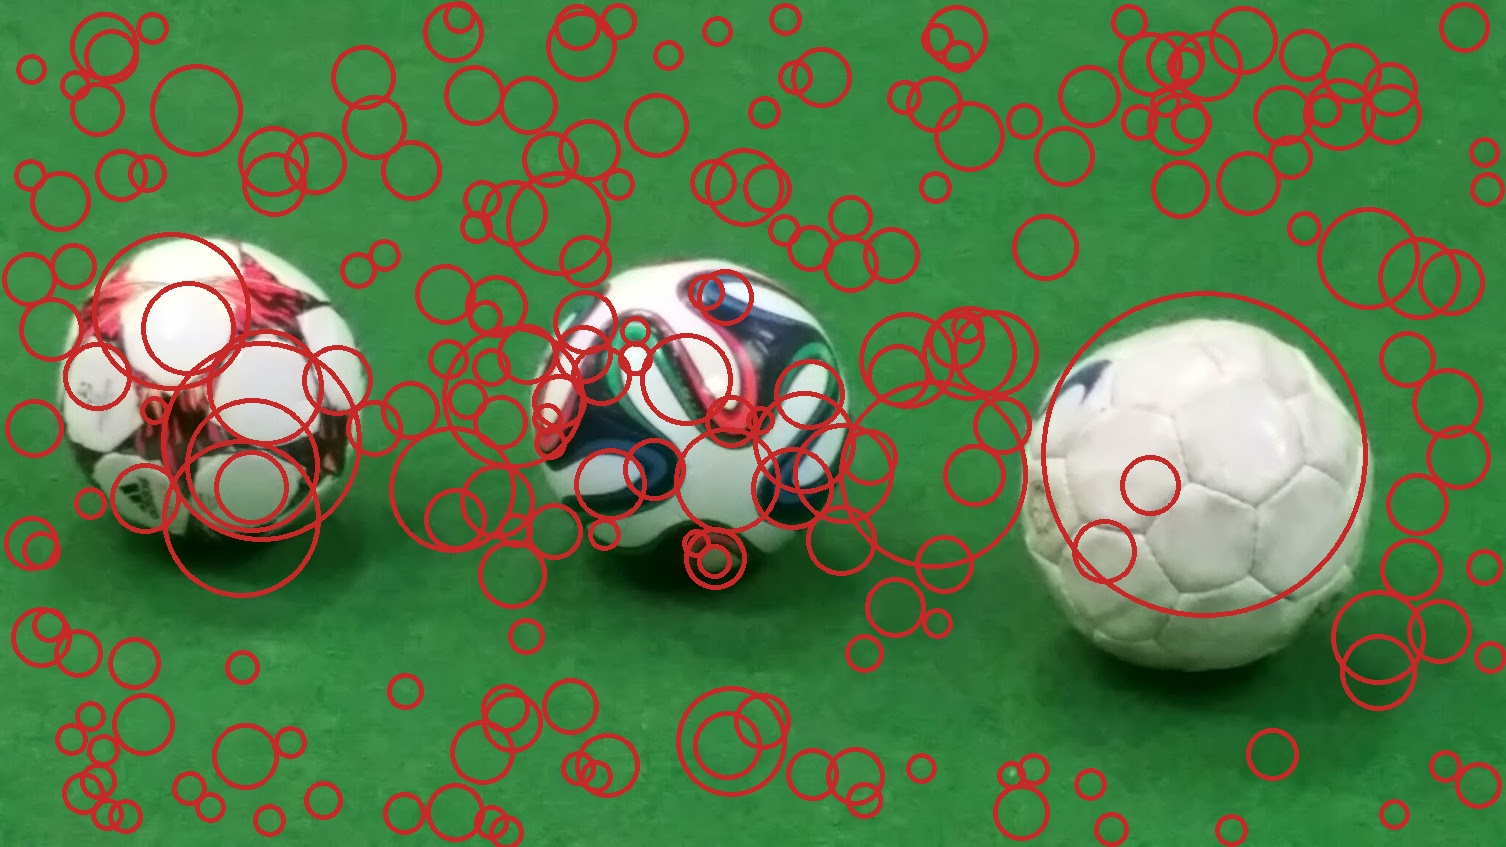
\includegraphics[width=6.0cm]{results/3/sphere_5}
    } \\
    \multicolumn{5}{c}{
        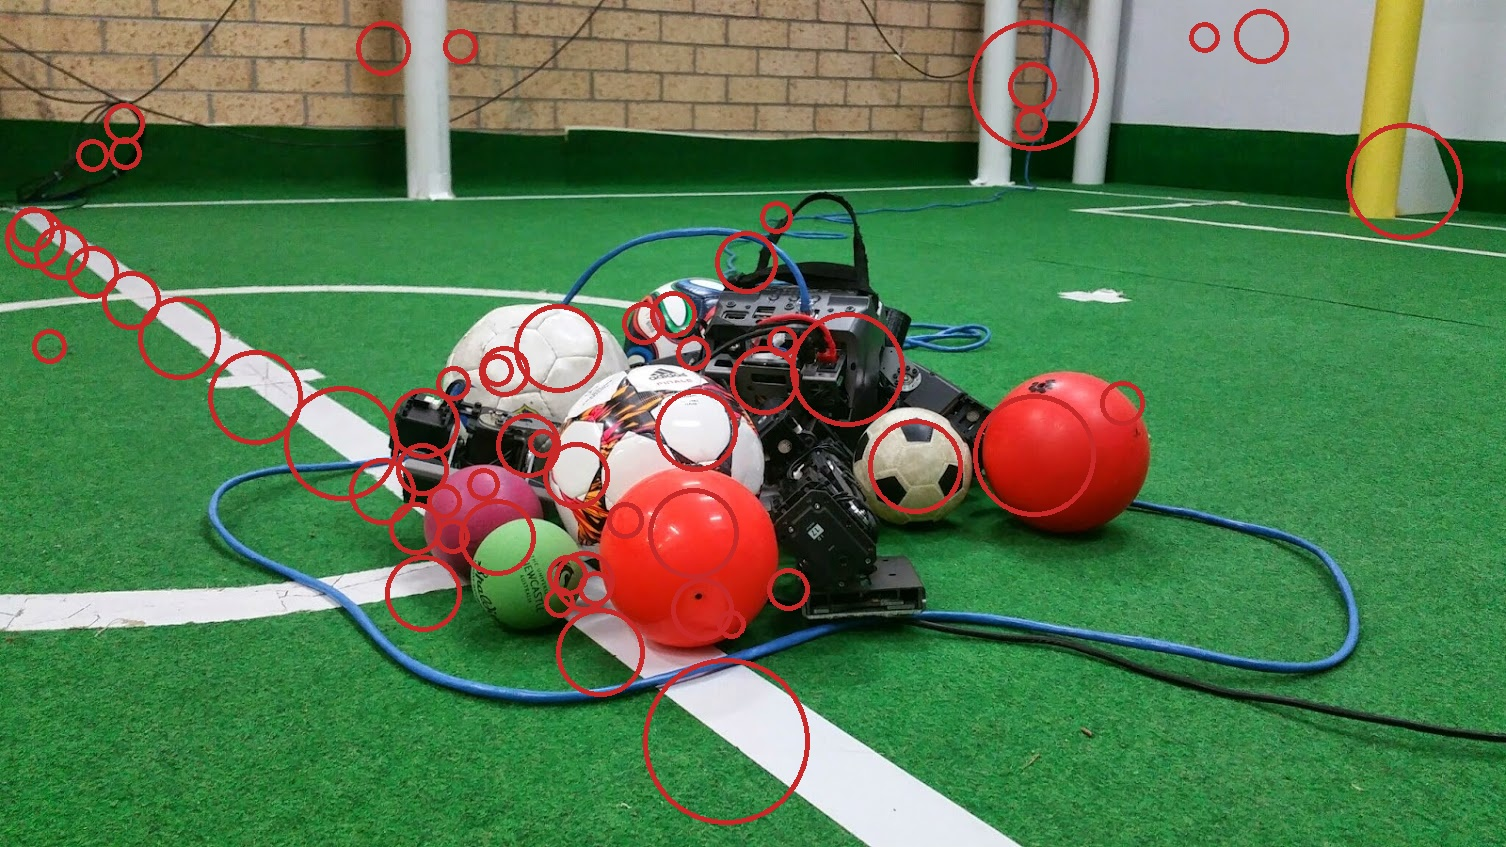
\includegraphics[width=6.0cm]{results/3/sphere_6}
        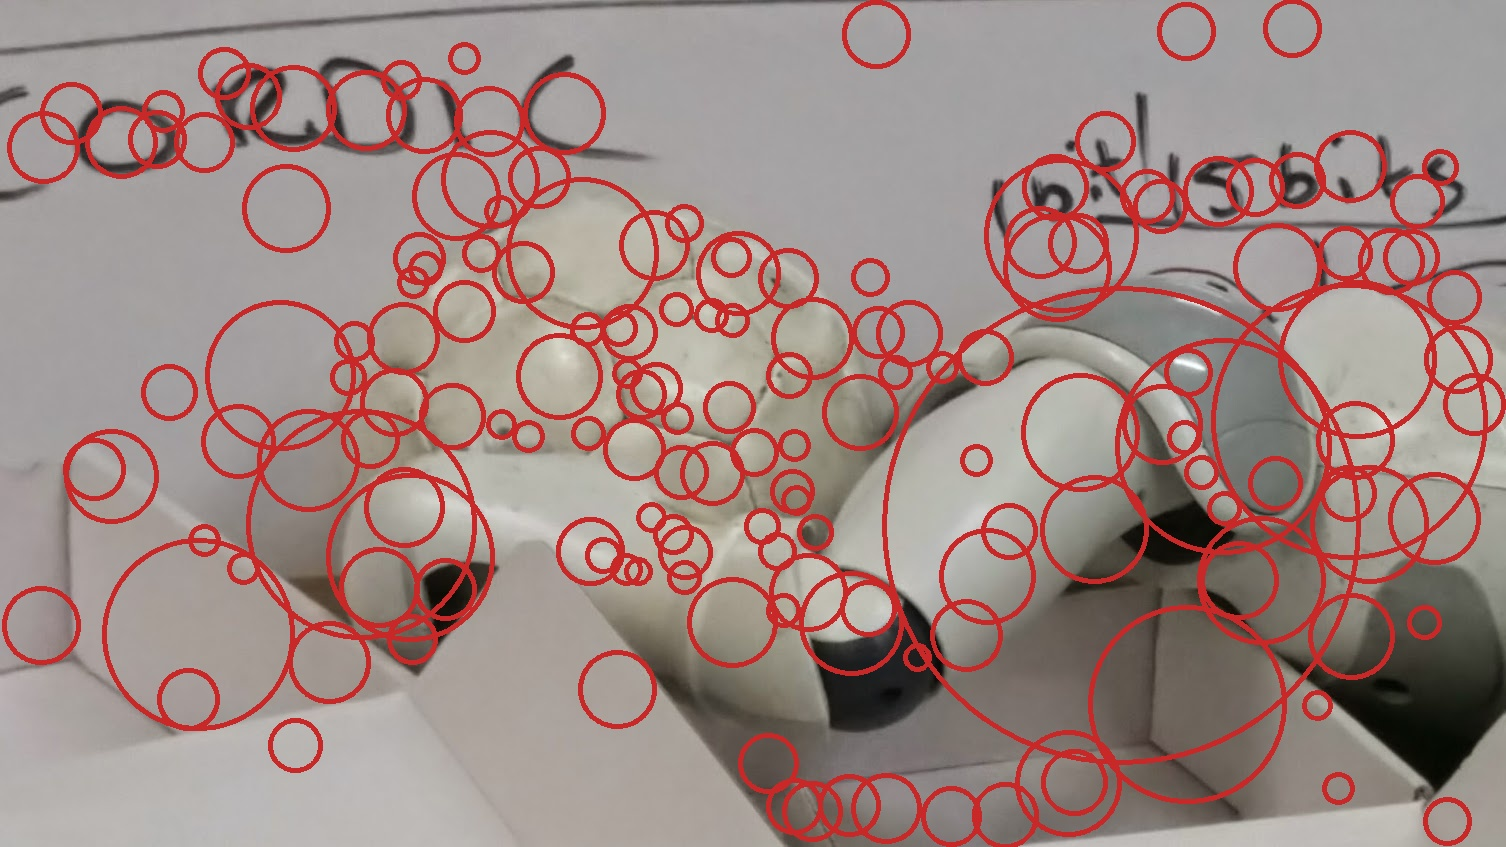
\includegraphics[width=6.0cm]{results/3/sphere_7}
        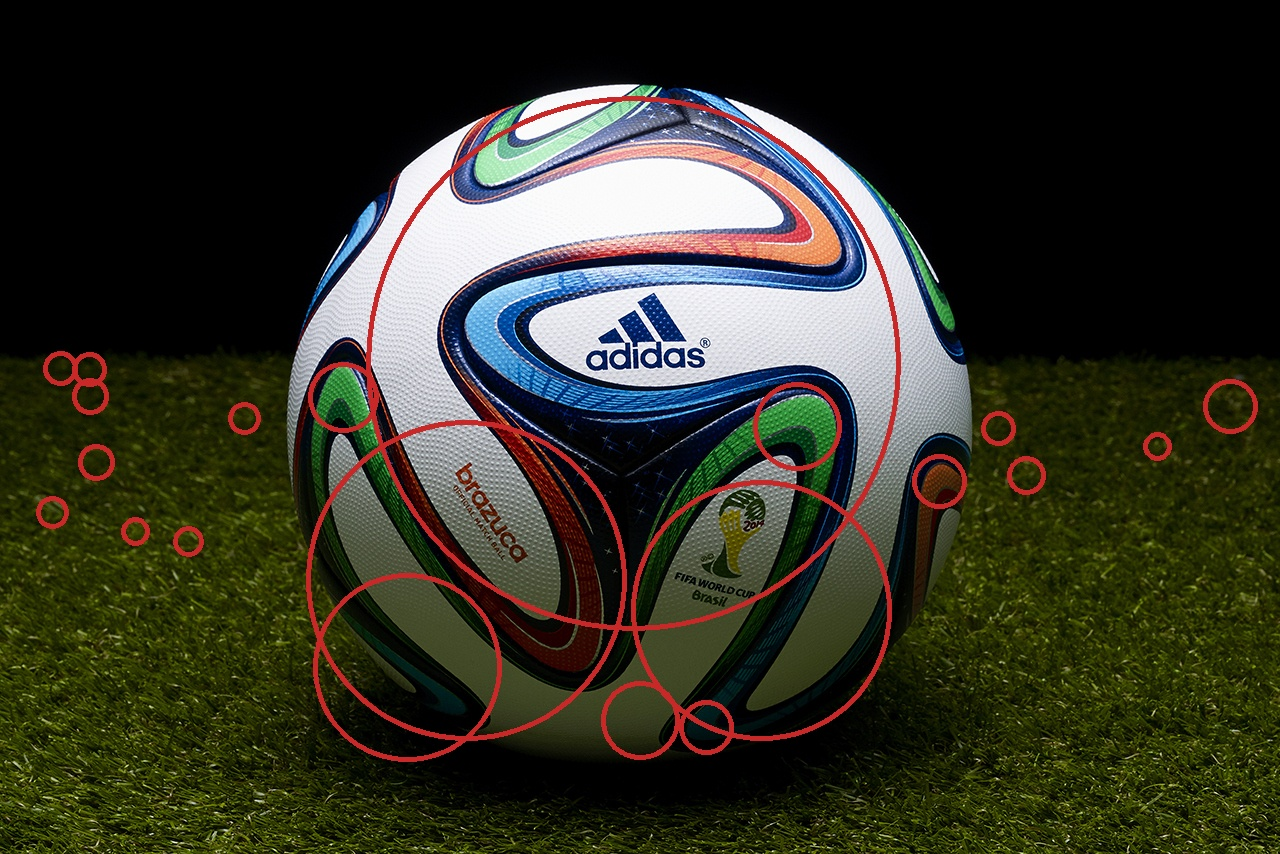
\includegraphics[width=6.0cm]{results/3/sphere_8}
    } \\
    % \bottomrule
\end{tabularx}
